\documentclass[a4paper,10pt]{article}
%\documentclass[a4paper,10pt]{scrartcl}

\usepackage[utf8]{inputenc}
\usepackage[shortlabels]{enumitem}
\usepackage{hyperref}
\usepackage{tabularx}
\usepackage{booktabs}
\usepackage{float}
\usepackage{longtable}

\usepackage{graphicx}
\graphicspath{{images/}}

\usepackage{geometry}
\geometry {
    top=20mm
}

\title{Economics of Cyber Security \\
  Individual Assignment  \\
  \large Group 8 (IoT Honeypots)}
\author{
  Yoep Kortekaas \\ 
  s1719734 (UTwente) \\
  4984595 (TUDelft)
}
\date{\today}

\begin{document}

\maketitle

\begin{abstract}
% Abstract - The abstract should be no longer than 100 to 150 words. It should convey the topic and research question, the hypothesis, 
% the key findings and key discussion points – all within the 150 word limit.
In this research, we look at IoT botnets and whether they are used for cyber criminal activities other than generating DDoS attacks. 
For this we compare the IP addresses of  known infected IoT devices with IP addresses found in spam, phishing and malicious executable hosting data 
sets. Our main research question is "Are infected IoT devices used for other types of cyber crime than just DDoS attacks?" with main 
hypothesis that yes, infected IoT devices are used for other types of cyber crime than just DDoS attacks. Our findings are that a 
statistical significant amount of infected IoT devices \textit{are} used for sending spam emails, but this is not the case for hosting 
phishing sites and malicious executables. In future research we would like to look at involvement of IoT botnets and infected IoT 
devices in other fields of cyber crime, such as blackmailing.
\end{abstract}

\section{Introduction} \label{sec:introduction}
% Introduction -  The introduction/justification and purpose section includes the background information on the security 
% issue and its importance.
Internet of Things (IoT) devices have been gaining popularity the last few years. According to a recent survey by Statista 
\cite{amount_iot_devices}, in 2016 there were 17.68 billion connected IoT devices installed worldwide. It is expected that in 2025 
there will be more than 75 billion IoT devices installed that are connected. These IoT devices are small, cheap, and have
huge potential to make common household items, such as for example thermostats, light switches, and power sockets, 
"smart" and connected to the internet.While these IoT devices sound like a match made in heaven for anyone who wants to get more insight in their exact 
electricity usage, or when you want to toggle the lights without getting out of bed, these cheap, low-power devices  are 
a nightmare in the world of cyber security.
\\\\
The 19th of September, 2016, the first ever Distributed Denial of Service (DDoS) attack with a magnitude of over 1 terrabit
per second (Tbps) was recorded, when French hosting provider OVH was hit with a DDoS attack of 1.1 Tbps \cite{ovh}. 
According to the CEO of OVH, the DDoS attacks were produced by a collection of millions of hacked IoT devices, mostly
internet-connected camera's and digital video recorders. This would be the first in a series of DDoS attacks of this 
magnitude that OVH would experience. The cause of these hacked IoT devices? Bad security practices.
\\\\
The botnet of IoT devices that attacked OVH were infected with a malware named 'Mirai'. The way Mirai infected these
devices was quite simple, it connected to a device, and tried to log in using a list of default username/password credentials
\cite{how_mirai_works} No complicated zero-day exploits or other hacks, just trying out default log-in credentials. IoT 
devices are usually very  simple devices. It does not take a lot of effort for a manufacturer to develop IoT devices, 
meaning that to make a profit, new types IoT devices need to be quickly, and as cheap as possible. 
\\\\
Developing cheap devices usually also  means that there is little to no budget for 
security. Furthermore there is also little incentive for IoT device manufacturers to invest in security. The manufacturers 
of the IoT devices are usually not the targets of the DDoS attacks that are generated by their devices, just like the 
customers that they are targeting are (usually) not the victims of DDoS attacks, and most customers won't even notice
that their devices have been breached! And if a customer is not aware of the impact of the (lack of) security of their IoT device,
why would they pay more for a more secure IoT device with the same functionality?
\\\\
In this report we will review current research on the security issue, vulnerable IoT devices and (IoT) botnets, in \autoref{sec:literature_review}. We will follow up with
defining our own research questions and hypotheses in \autoref{sec:research_questions}. In \autoref{sec:methodology} we
describe how we will answer the research questions, and test the hypotheses. \autoref{sec:results} will contain the results
of our research, followed by the limitations of our research in \autoref{sec:limitations}. Finally we will conclude in 
\autoref{sec:conclusions}.

\section{Literature Review} \label{sec:literature_review}
% Literature Review - The literature review is a summary of the pertinent, existing research on the security issue under 
% investigation. Please include a discussion of 5 high quality peer-reviewed references related to your security issue.
% Oftentimes the literature review will provide evidence for the types of variables selected as well as a review of what 
% research has already been done and what still remains to be done for the context and research question selected.
% 
% https://www.semanticscholar.org/paper/Botnets-and-Internet-of-Things-Security/7ec61ba81a7707e5a06591c984a0660719340d8a
In this section we will discuss five different existing works that look at the security issue we discussed in 
\autoref{sec:introduction}. 

\subsection{Turning Internet of Things(IoT) into Internet of Vulnerabilities (IoV) : IoT Botnets} \label{sec:literature_review:angrishi2017}
In \cite{angrishi2017turning}, Angrishi looks at an outline of the structure of IoT botnets, and how they operate. Angrishi
identifies that botnets have two core components, namely \textit{Bots} that perform DDoS attacks on demand, and
\textit{Command and Control servers} that are used to control the bots. Additionally, IoT botnets also contain 
\textit{Scanners} that are used to scan for vulnerable devices, \textit{Reporting servers} that are used to collect reports
on the bots in the network, \textit{Loaders} that are used to log on vulnerable devices and let them download malware,
and \textit{Malware distribution servers} where the malware code that vulnerable devices download is stored.
\\\\
Next to looking at the structure of IoT botnets, Angrishi also looks at notable IoT incidents, and identifies possible
remedies, as well as defining some security best-practices for IoT device owners.  Some of the remedies Angrishi 
recommends are:
\begin{itemize}
 \item Limiting network communication of IoT devices to the website/IP of the manufacturer
 \item A unique, random, default password per IoT device
 \item IoT device manufacturers should be held accountable for following and implementing security best-practices
 on their devices.
\end{itemize}

\noindent Some of the best security practices for IoT devices that Angrishi identifies are:
\begin{itemize}
 \item Changing the default password of their device
 \item Always update their IoT devices with security updates as soon as they are made available
 \item Only purchasing IoT devices from manufacturers that have a good track record for producing secure
 devices and responding to incidents with regular security updates.
\end{itemize}

\subsection{{DDoS} in the {IoT}: Mirai and Other Botnets} \label{sec:literature_review:kolias2017}
In \cite{Kolias2017}, Kolias et al. look at the Mirai botnet, its main components, how it operates and how it communicates.
Furthermore they also look at Mirai variants and other IoT botnets, and identify five main reasons why IoT devices are
advantageous for creating IoT botnets.
\\\\
Kolias et al. identify four main components in the Mirai botnet. The \textit{Bots} are the infected IoT devices, the 
\textit{Command and Control server} provides the botmaster with a centralized management interface for 
orchestrating new DDoS attacks, the \textit{loader} facilitates broadcasting of malware executables to new victims, and
finally the \textit{Report server} maintains a database with details about all bots in the botnet. Kolias et al. also identify 
seven steps in the communication and operation of the Mirai botnet, which can be found in \autoref{fig:kolias_communication}.

\begin{figure}[hbtp]
 \centering
 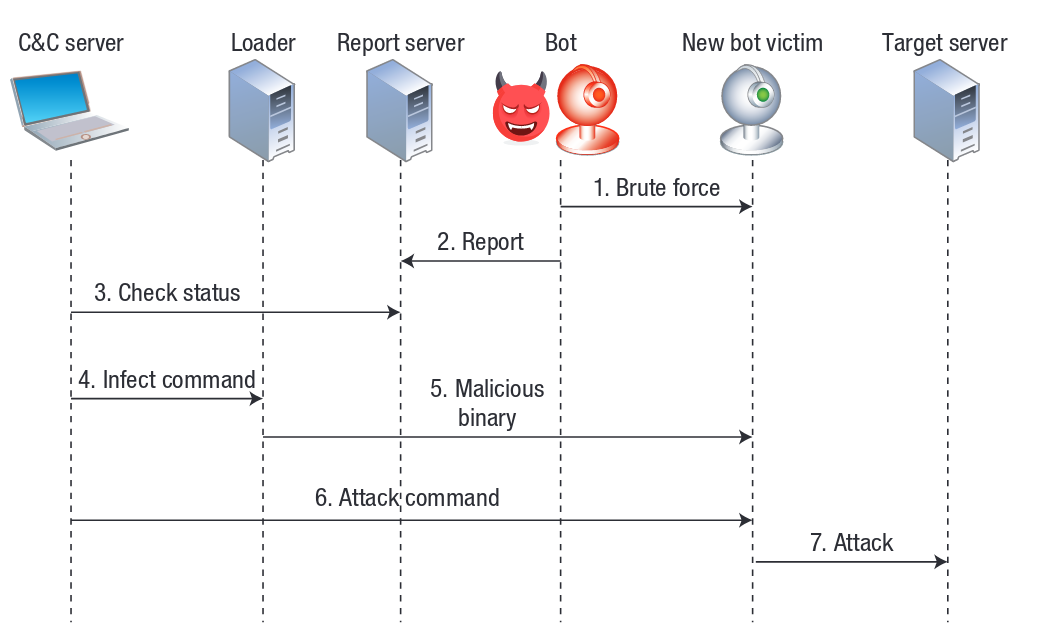
\includegraphics[width=0.8\linewidth]{kolias.png}
 \caption{Communication and operation of the Mirai botnet identified by Kolias et al. in \cite{Kolias2017}}
 \label{fig:kolias_communication}
\end{figure}
~\\
Kolias et al. identify several Mirai variants, that for example use different ports than Mirai, or that install crypto currency
miners on infected devices. They also identify more sophisticated IoT botnets that can infect more devices, and actually
try to obfuscate their activity, through the use of encrypted command and control communication. They have also 
identified botnets that communicate through decentralized means, instead of through a centralized command and 
control server.
\\\\
Finally, the five main reasons why it is attractive to target IoT devices for botnets that Kolias et al. have identified are:
\begin{itemize}
 \item \textit{Constant and unobtrusive operation} - Many IoT devices run 24/7, unlike most laptops and desktop 
 computers.
 \item \textit{Feeble protection} - Many IoT device vendors in the rush to penetrate the IoT market neglect security
 \item \textit{Poor maintenance} - Most IoT devices are forgotten once they are set-up, as long as they keep functioning
 \item \textit{Considerable attack traffic} - Most IoT devices are powerful enough to produce DDoS traffic comparable 
 to a laptop or desktop pc.
 \item \textit{Non-interactive or minimally-interactive user interfaces} - Since IoT devices are meant to have little user 
 intervention, infections are more likely to go unnoticed. When they \textit{are} noticed, there is no easy way for an user
 to address the issue, other than replacing the device.
\end{itemize}

\subsection{IoT security: Review, blockchain solutions, and open challenges} \label{sec:literature_review:khan2018}
In \cite{Khan2018}, Khan et al. discuss popular IoT security issues, and outline several security requirements for IoT along
with attacks, threats and solutions. Khan et al. also discuss how blockchain technology can help in solving many of the 
IoT security problems. 
\\\\
Khan et al. identify in total 19 different security issues in IoT, and categorize them in low-level, intermediate-level and 
high-level security issues. For each of the security issues they identify, also a proposed solution is mentioned. An excerpt
of this can be seen in \autoref{fig:khan_solutions}.

\begin{figure}[hbtp]
 \centering
 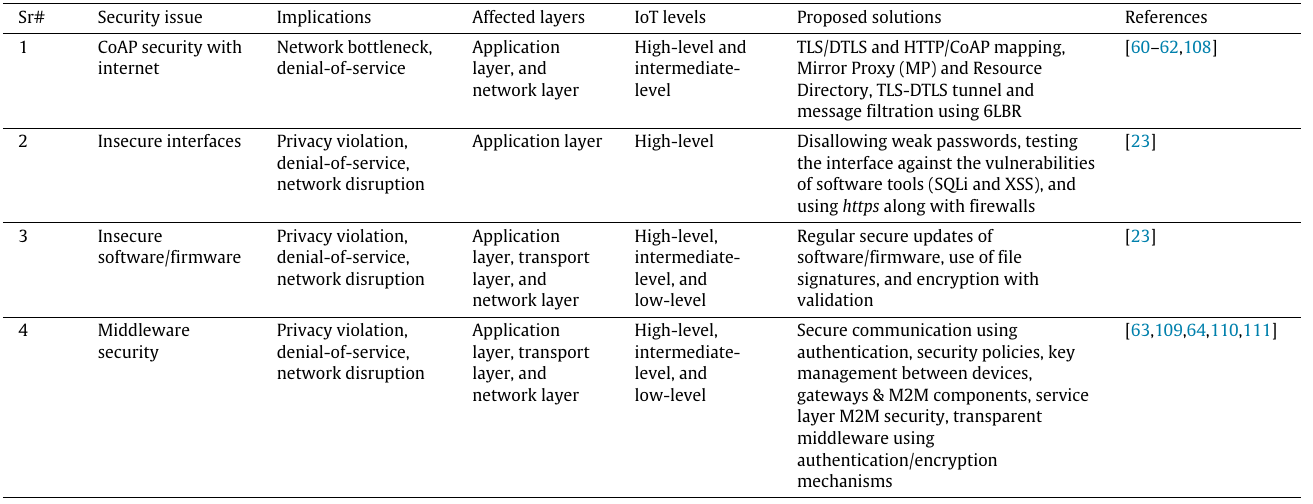
\includegraphics[width=\linewidth]{khan.png}
 \caption{Mapping of high-level security issues, implications and solutions identified in \cite{Khan2018}}
 \label{fig:khan_solutions}
\end{figure}

According to Khan et al. blockchain can help IoT security issues in a few different ways. Blockchain can help with the 
limited \textit{address space}, (160 bits of address space instead of the 128 bits of IPv6), with \textit{ identity management 
and governance}, with \textit{data authentication and integrity}, with \textit{authentication, authorization and privacy}, 
and with \textit{secure communications}.

% Scrapped for now
% \subsection{The Effect of IoT New Features on Security and Privacy: New Threats, Existing Solutions, and Challenges Yet to Be Solved} \label{sec:literature_review:zhou2019}
% In \cite{Zhou2019}, Zhou et al. introduce the concept of "IoT features", and discuss the security and privacy effects of 
% eight of these IoT features. IoT features refer to the unique features of IoT devices, network, and applications.
% \\\\
% The eight IoT features, accompanied with  that Zhou et al. identify are: Interdependence, Diversity, Constrained, Myriad, 
% Unattended, Intimacy, Mobile, and Ubiquitous. These features are not independent, but interact with and influence each
% other. An overview of all features, threats, challenges and opportunities can be found in \autoref{fig:zhou_features}
% 
% \begin{figure}[hbtp]
%  \centering
%  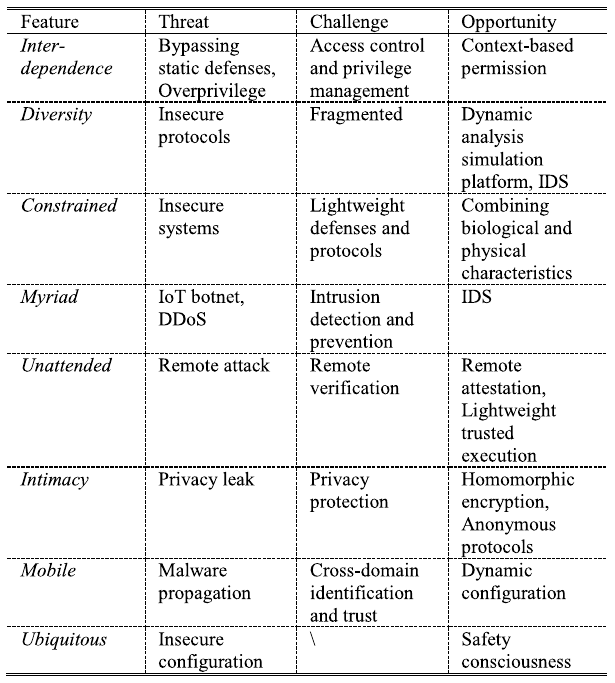
\includegraphics[width=0.45\linewidth]{zhou.png}
%  \caption{IoT feature, threats, challenges and opportunities identified in \cite{Zhou2019}}
%  \label{fig:zhou_features}
% \end{figure}
% ~\\
% Lastly, Zhou et al. analyze previous research on IoT security, and illustrate the development trend and how their defined
% IoT features reflect on the previous research, in order to identify IoT security research directions and priorities.

\subsection{A Taxonomy of Botnet Behavior, Detection, and Defense} \label{sec:literature_review:Khattak2014}
In \cite{Khattak2014}, Khattak et al. look existing botnet literature, and structure that in three different categories/
taxonomies, botnet behavioral features, botnet detection and botnet defenses, highlighting per category areas where
further research is needed. Khattak et al. do not exclusively look at IoT based botnets, but look at botnets in general.
\\\\
In the taxonomy of botnet behavior, Khattak et al. classify botnets based on their behavior. The behavioral features
that Khattak et al. focus on concern \textit{Propagation}, \textit{Rallying}, \textit{Command \& Control}, \textit{Purpose},
and \textit{Evasion}. The full taxonomy of botnet behavioral features can be found in \autoref{fig:khattak_behavior}.

\begin{figure}[hbtp]
 \centering
 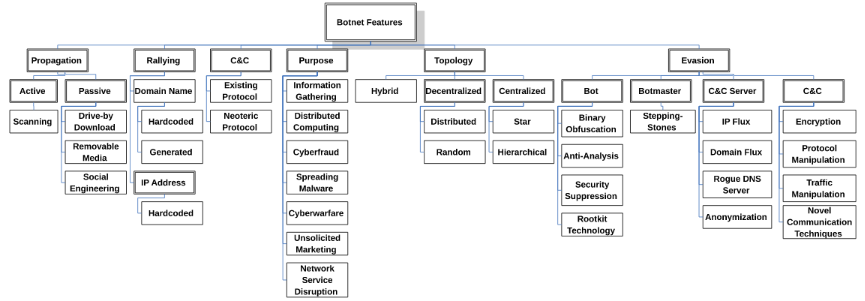
\includegraphics[width=0.9\linewidth]{khattak-behavior.png}
 \caption{The botnet-behavior-based taxonomy described in \cite{Khattak2014}}
 \label{fig:khattak_behavior}
\end{figure}
~\\
In the taxonomy of botnet detection, Khattak et al. classify different approaches of botnet detection. Khattak et al. 
split the detection methods up in three different facets, namely \textit{bot detection}, \textit{Command \& Control
detection}, and \textit{botmaster detection}. Furthermore, these facets are again split up in \textit{Active} and 
\textit{Passive} detection methods, since while active methods are usually more effective, they usually also raise
ethical and legal issues. The full taxonomy of botnet detection methods can be found in \autoref{fig:khattak_detection}.
\\
\begin{figure}[hbtp]
 \centering
 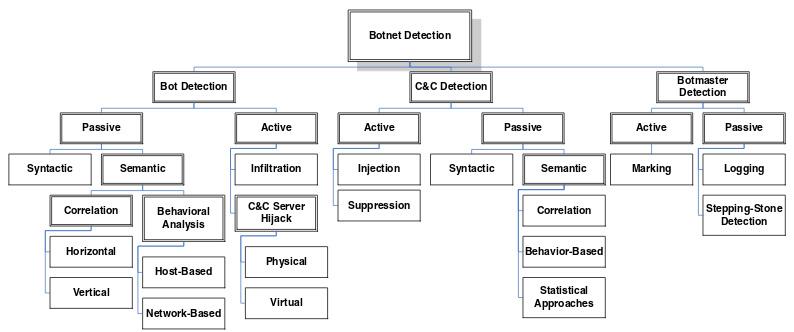
\includegraphics[width=0.9\linewidth]{khattak-detection.png}
 \caption{The detection method-based taxonomy described in \cite{Khattak2014}}
 \label{fig:khattak_detection}
\end{figure}

\noindent As seen in the taxonomy of botnet detection, Khattak et al. split each facet up in \textit{Active} and \textit{Passive}
methods; they classified along the \textit{dimension} 'level of activity'. According to Khattak et al., these botnets can be
classified along a lot more, different dimensions. All dimensions Khattak et al. identify as being interesting to look at
are: \textit{Specificity}, \textit{Discernment}, \textit{Mode of Operation}, \textit{Location of Deployment}, \textit{Level of
Activity}, \textit{Degree of Automation}, \textit{Analysis Direction}, and \textit{Analysis Depth}.
\\\\
In the taxonomy of botnet defense strategies, Khattak et al. classify different methods of defense against infection.
The strategies are categorized in two different categories, namely \textit{Preventive} strategies and \textit{Remedial}
strategies. Preventive strategies concern the avoidance of botnet infection, and remedial strategies concern themselves
with the cleaning of the system once an infection has happened. In the preventive category the defense mechanisms have
been split up in \textit{Technical} and \textit{Non-Technical} approaches, and in the remedial category the defense mechanisms
have been split up in \textit{Defensive} and \textit{Offensive} approaches. The full taxonomy of botnet defense strategies can 
be found in \autoref{fig:khattak_defense}.
\\
\begin{figure}[hbtp]
 \centering
 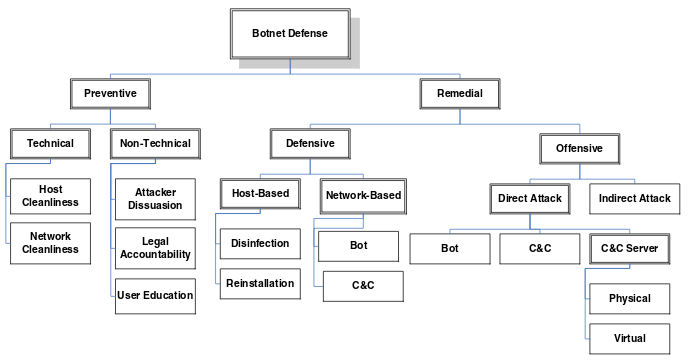
\includegraphics[width=0.9\linewidth]{khattak-defense.png}
 \caption{The defense strategy-based taxonomy described in \cite{Khattak2014}}
 \label{fig:khattak_defense}
\end{figure}

\subsection{Motivating a market or regulatory solution to {IoT} insecurity with the Mirai botnet code} \label{sec:literature_review:Jerkins2017}
In \cite{Jerkins2017}, Jerkins proposes a way to motivate IoT device operators to address poor security practices. Jerkins
identify an absence of market or social forces to motivate Internet Service Providers (ISPs), manufacturers and IoT
device owners to resolve the security issue of IoT devices. Therefore, according to Jerkins, the government should
provide incentives to resolve the issue through regulatory means. 
\\\\
To help regulatory instances regulate the market, Jerkins modified the open sourced Mirai botnet source code. The
modified malware identifies vulnerable devices, stores information about the vulnerable devices in a central database, 
and sends the network operator of the network the IoT device is connected to an email stating the vulnerability.  
Periodically, the modified command and control server will generate a report containing the amount of vulnerable 
devices per IoT device manufacturer. A written notification can then be send to the manufacturer by the appropriate 
governmental authority.

% https://www.usenix.org/conference/hotedge18/presentation/bhardwaj
% https://www.computer.org/csdl/magazine/co/2017/02/mco2017020076/13rRUxZRbvu
% https://dl.acm.org/citation.cfm?id=2691450 - CAD paper

\section{Research Questions, Objective, and Hypothesis} \label{sec:research_questions}
% o Postulate and state a relevant research question in economics of cybersecurity related to the dataset
%     you have used during the previous assignments. 
% 
% o State a substantive hypothesis based on your research question that can be tested with the data/metrics
%     that you have developed during the group assignments (or further metrics, if you so desire), where
%     needed complemented by additional metrics/datasets as explanatory factors.  Make sure you show how 
%     the hypothesis is related to your literature review.
In \autoref{sec:literature_review} we looked at five different pieces of literature related to the security of IoT 
devices, IoT malware like Mirai, the involvement of IoT devices in DDoS attacks, botnets in general, and how 
to motivate a market to improve IoT security with a regulatory solution.
\\\\
The literature we looked at mostly focused on IoT device involvement in DDoS attacks. But as seen in \cite{Khattak2014},
botnets (and thus also IoT botnets) can be used for a lot more than just generating DDoS attacks. According to Khattak et. al
in \cite{Khattak2014}, they can also be used for information gathering, distributed computing, cyber fraud (such as phishing),
spreading malware, cyberwarfare, and unsolicited marketing (e.g. sending spam mails).
\\\\
In this research we want to get a better grasp on how IoT bot(net)s are used, and what kind of threat they really are to the 
outside world, so that we can better justify current spending on IoT security and IoT botnet prevention, and if there is a
serious enough security issue, even
justify an increase of IoT security spending. For this we take a look at a subset of the botnet purposes defined by Khattak et al., and
we look at use of IoT bot(net)s in unsolicited marketing, cyber fraud and spreading malware. When researching this, we 
asked ourselves the following research questions:
\begin{enumerate}
 \item[] \textbf{RQ1}: Are infected IoT devices used for other types of cyber crime than just DDoS attacks? \label{rq1}
 \begin{enumerate}
  \item[] \textbf{RQ1.1}: Are infected IoT devices used to send spam emails? \label{rq11}
  \item[] \textbf{RQ1.2}: Are infected IoT devices used to host malicious websites? \label{rq12}
  \item[] \textbf{RQ1.3}: Are infected IoT devices used to host malicious executables? \label{rq13}
 \end{enumerate}
\end{enumerate}
~\\
Before we answer these research questions, we of course have some expectations of the outcome of our research.
Since sending spam emails and hosting malicious websites (e.g. phishing websites) are very common 
\cite{common_cyber_crime},  simple/approachable forms of cyber crime, we expect that a significant amount of 
infected IoT bots are also used in these types of cyber crime. Since making malware/malicious executables, and actually
infecting devices with malware is more difficult than sending spam / hosting phishing sites, we expect that there will not
be a significant amount of IoT bots that are used for hosting malicious executables. Therefore, our hypotheses for this 
research are that:
\begin{itemize}
  \item[] \textbf{H1}: Infected IoT devices are used for other types of cyber crime than just DDoS attacks.
  \begin{itemize}
    \item[] \textbf{H1.1} A statistically significant amount of infected IoT devices are used to send spam emails.
    \item[] \textbf{H1.2} A statistically significant amount of infected IoT devices are used to host malicious websites.
    \item[] \textbf{H1.3} A statistically \textit{in}significant amount of infected IoT devices are used to host malicious 
    executables.
  \end{itemize}
\end{itemize}

\section{Methodology} \label{sec:methodology}
% Methodology (Research Design) - Describe the research method (qualitative or quantitative, or a combination 
% thereof, descriptive, explanatory) and statistical technique (comparison of means, regression analysis, etc.) that 
% you will use to answer your research question and test your hypotheses. 
\subsection{Data Sets} \label{sec:methodology:data}
In order to research \textbf{RQ1}, \textbf{RQ1.1}, \textbf{RQ1.2}, and \textbf{RQ1.3}, we will need some data.
First of all we need have an idea of what infected IoT devices are, and how many there are. For that we have
an IoT honeypot data set \cite{iot_honeypot_dataset}. This data set contains 47 days of recorded malicious traffic 
IoT botnet traffic. This data set recorded per connection it received: a timestamp, source IP/port of the infected IoT 
device, destination IP/port in the honeypot, and a list of commands that the infected source tried to execute. This 
data set will give us a baseline of which IPs we encounter are vulnerable IoT devices.
\\\\
To answer \textbf{RQ1.1}, we will need to know which devices / IP addresses generate spam emails. For this we
will use an email spam blacklist. The spam blacklist we have chosen to use is the Spamhaus Zen blacklist 
\cite{spamhaus_zen}. The Spamhaus ZEN blacklist is one of the most widely used blacklists for determining whether 
an IP address is malicious with regard to sending spam or not.
\\\\
To answer \textbf{RQ1.2}, we will need to know which URLs / IP addresses are hosting phishing sites. For this we
are using the Phishtank phishing domain data set \cite{phishtank}. According to the FAQ hosted on the Phishtank website,
"PhishTank is a free community site where anyone can submit, verify, track and share phishing data"\footnote{\url{https://www.phishtank.com/faq.php\#whatisphishtank}}. The Phishtank
data set contains a lot of information regarding phishing URLs, such as the phishing site URL, the submission time,
whether the URL has been verified as actual phishing site, the IP address of the malicious URL and the phishing target.
For this research we will only use the submission time and IP address of verified phishing URLs.
\\\\
To answer \textbf{RQ1.3}, we will need to know which URLs / IP addresses are hosting malicious executables. For 
this we are using two different sources, \url{malwaredomainlist.com} \cite{malwaredomainlist} and 
\url{malc0de.com} \cite{malc0de}, since the amount of IPs / hosts used for distributing malware is relatively
low. A small issue with the malc0de data set, is that it only stores the last 30 days of malicious IPs. So to in order to 
download a more complete IP blacklist of the malc0de data set, we downloaded with the help of the Internet Archive's
"Wayback Machine"\footnote{\url{https://archive.org/web/web.php}}, all blacklists starting from June 2016
up until now, and combined that into one big IP blacklist.

\subsection{Statistical Analysis} \label{sec:methodology:stat_analysis}
With the data collected from \autoref{sec:methodology:data}, we actually make some conclusions about our data.
For answering \textbf{RQ1.1}, \textbf{RQ1.2}, and \textbf{RQ1.3}, respectively testing \textbf{H1.1}, \textbf{H1.2}, 
and \textbf{H1.3}, the process looks roughly the same. We assume that the botnet owners choose infected IoT bots 
that are used for sending spam emails / hosting phishing sites / hosting malicious malware executables at random.
There always is a (albeit low) probability that a few IP addresses in the data sets that we are comparing with are from 
infected IoT devices, that have not been instructed by the botnet owner to do these malicious actions. We estimate 
that this is the case with a probability of approximately 0.5\% of the vulnerable IoT devices. Since there is a difference 
in the amount of unique IP addresses/devices in our data set per day, we take the day with the highest amount of unique 
IPs (40158) connecting to the honeypot to be on the safe side in our statistics calculation.
\\\\
Since we assume that the infected IoT devices that are in the spam, phishing and malicious executable data sets, 
and the infected IoT devices that the bot owners choose to do their dirty work are randomly chosen with probability
$p = 0.005$, we can approximate this binomial distribution with a normal distribution. With the amount of devices
we have, $n = 40158$, and our probability we can verify that $n \cdot p \geq 25$ and $n \cdot (1-p) \geq 25$, and
thus we can approximate the distribution with a normal distribution with $\mu = n \cdot p = 200.79$ and 
$\sigma = \sqrt{n \cdot p \cdot (1-p)} \approx 14.13$. We will also compare percentages of devices that are
in the spam / phishing / malicious executable data set, and in this case we take a normal distribution with 
$\mu = p =0.005$ and  $\sigma = p \cdot (1-p) = 0.004975$.
\\\\
We then use a both a T-test and a Mann-Whitney U test to verify our hypotheses and to  test whether the amount 
of IoT bots used for sending spam emails / hosting phishing sites / hosting malicious malware executables are 
significantly higher than the 0.5\% that we expected to see. We use both a T-test and Mann-Whitney U test,
since we then still can have statistically significant results in the case our normality assumption was incorrect.
\\\\
When we have answered and tested \textbf{RQ1.1} and \textbf{H1.1}, \textbf{RQ1.2} and \textbf{H1.2}, and 
\textbf{RQ1.3} and \textbf{H1.3}, we can also answer \textbf{RQ1} and \textbf{H1}, since their answers
depend on the results we get when answering the sub-research questions and sub-hypotheses.

% Other data sets with nice data that we won't be using:
% Blocklist.de - Not specific for rqs
% hpHosts - No IPs
% CleanMX - no API key/user agent

\section{Results} \label{sec:results}
% o Describe the findings from your study. Include and discuss the results of your statistical test. For each;
% o Include the relevant statistical output (e.g., ANOVA table, etc.) or a chart, figure, or graphs that illustrates
%     your results. Do not include long frequency distributions or extraneous tables and figures that do not 
%     support your findings.
% o Discuss and interpret each result. This includes which hypothesis you supported and describe what 
%     supporting that hypothesis means.
% o Explain what you think the statistical results imply.

In the appendix in \autoref{tbl:results_full} the results of our experiment can be seen, an excerpt of that table can be seen in 
\autoref{tbl:results_partial}. The first most obvious thing to notice are the
columns for the \textit{Phishtank} data set and \textit{Malc0de and Malwaredomainlist} data set. These columns 
have all zero values, meaning than none of the IP addresses of the vulnerable IoT devices found in our IoT honeypot 
data set have been found in the \textit{Phishtank}, \textit{Malc0de} or \textit{Malwaredomainlist} data sets. 
\\\\
There can be multiple different explanations for these zero columns. The first explanation is that these devices we have
in our IoT honeypot data set have never been used for hosting phishing sites or malicious executables, or maybe they have
not even been used for any other thing than expanding the botnet and performing DDoS attacks. The latter seems unlikely, 
since we do get hits from the Spamhaus ZEN data set, but the former could be the case. 
\\\\
A different explanation could be that our data sets are incomplete. While this could be the case  for the Malc0de and
Malwaredomainlist data sets, since with their respective sizes of 2345 and 997 entries the combined data set is quite small, this seems unlikely for the
PhishTank data set with over 500,000 entries.  Therefore we deem it possible that we just had "bad luck" with our
Malc0de and Malwaredomainlist data sets, but the fact that none of the IoT botnet IPs are in the Phishtank data set 
cannot be explained by luck/chance.

\begin{table}[h]
%  \centering
 \begin{tabularx}{\linewidth}{lXXXXXX}
 \toprule
 File & Spamhaus ZEN (\#) & Spamhaus ZEN (\%) & Phishtank (\#) &  Phishtank (\%) & Malc0de and Mdl (\#) & Malc0de and Mdl (\%) \\
 \midrule
 2016-07-01.csv & 411 & 1.59 & 0 & 0.00 & 0 & 0.00 \\
 2016-07-02.csv & 517 & 1.84 & 0 & 0.00 & 0 & 0.00 \\
 &  &  & $\vdots$ &  &  &  \\
2016-09-12.csv & 173 & 1.49 & 0 & 0.00 & 0 & 0.00 \\
2016-09-13.csv & 152 & 1.53 & 0 & 0.00 & 0 & 0.00 \\
 \bottomrule
 \end{tabularx}
 \caption{Partial results of comparing the IP addresses of the infected IoT devices with the different collected data sets}
 \label{tbl:results_partial}
\end{table}
~\\
Looking at columns 2 and 3 however, we see that we do have some hits for our  infected IoT devices in the Spamhaus
ZEN data set. On average, 1.77\% of the infected IoT devices in our IoT honeypot data set are also on the Spamhaus ZEN
spam blacklist. As mentioned in \autoref{sec:methodology:stat_analysis}, we apply a T-test  and a Mann-Whitney U test
to verify whether the amount of devices we see in the Spamhaus data set is significant. 
\\\\
Since we have data about the exact number of devices and the percentages, we define two different null hypotheses, 
$H_0^{exact}$ and $H_0^{percent}$, and we define them as:
\begin{itemize}
 \item[] $H_0^{exact}:$ The amount of infected IoT devices sending spam emails is normally distributed with a mean 
 of 401.68 and  a standard deviation of 200.79.
 \item[] $H_0^{percent}:$ The amount of infected IoT devices sending spam emails is normally distributed with a mean 
 of 0.005 and  a standard deviation of 0.004975 .
\end{itemize}
~\\
The results we got for our statistical tests can be found in \autoref{tbl:stats_exact} and \autoref{tbl:stats_percent}. We 
can clearly see that in both the statistical tests with the exact number of IP addresses and the statistical tests with a 
percentage of the amount of IP addresses, that the p-values of the tests are strong enough to reject  $H_0^{exact}$ 
\textit{and} $H_0^{percent}$ ($p \leq 0.01$) in both the T-test and the Mann-Whitney U test.

\begin{table}[H]
    \centering
    \begin{minipage}{0.45\linewidth} \centering
        \begin{tabularx}{\linewidth}{p{0.29\linewidth}XX}
            \toprule
            Test & Test value & p-value  \\
            \midrule
            T-test & -4.888 & 1.336E-05 \\
            Mann-Whitney U test & 425.0 & 3.923E-07 \\
            \bottomrule
        \end{tabularx}
        \caption{Results of statistical tests with exact amount of IP addresses}
        \label{tbl:stats_exact}
    \end{minipage}
    \hspace{0.01\linewidth}
    \begin{minipage}{0.45\linewidth} \centering
        \begin{tabularx}{\linewidth}{p{0.32\linewidth}XX}
            \toprule
            Test & Test value & p-value  \\
            \midrule
            T-test & -16.46 & 1.162E-20 \\
            Mann-Whitney U test & 0.0 & 7.371E-17\\
            \bottomrule
        \end{tabularx}
        \caption{Results of statistical tests with percentage amount of IP addresses}
        \label{tbl:stats_percent}
    \end{minipage}
\end{table}


\section{Limitations} \label{sec:limitations}
% Limitations -  Assess the limitations of your research and discuss the recommendations for others who may research this topic 
% (i.e. what would you do differently?)
While we do believe that our research methodology described in \autoref{sec:methodology} is sound, there are of course always 
limitations that we run into during research. In this section we will describe those limitations, and  what we would like to have 
done different in an, albeit ideal, future research.
\\\\
The first limitation we would like to discuss is IP turnover. IP turnover is the concept that a lot of IP addresses are not static, but instead are
dynamically leased for a certain time period. Most home internet connections have dynamic IP addresses, meaning that they have
"ownership" of an IP address for a certain lease time, and after that lease time, for example 7 days, the lease has to be renewed. When
the lease is renewed, you can get a lease for the same IP again, but if it has already been taken you get another IP. The limitation
we came across is that while we can minimize the impact of IP turnover in the IoT honeypot data set, by looking only at the data of
one day at a time, this becomes more difficult for our other data sets. Therefore when we find an infected IoT IP in the other data sets,
we cannot be 100\% sure that the malicious behavior was generated by the IoT device or another malicious device that by chance
got the dynamic IP after the IoT device. Therefore in an ideal next research it would be good to have access to IP lease times in order
to get more accurate results, however we do acknowledge that this is probably infeasible.
\\\\
The second limitation we would like to discuss is the incompleteness of the data. While for example the Spamhaus ZEN and the 
Phishtank data sets contain a lot of entries, they probably do not have a complete overview of all malicious IP addresses with regard
to phishing and spam. Moreover, the Malc0de and Malwaredomainlist data sets are rather limited and are likely to miss a lot of 
hosts that host malicious executables. Therefore, in an ideal next research it would be better to have more complete data, especially
regarding the hosting of malicious executables. Some feasible improvements for the spam and phishing data sets can be made by 
looking at other data sets that only store malicious URLs, and performing DNS queries for those URLs to find out the malicious IPs.
Issues with this approach are however that the IP for an URL might change, for example due to IP turnover or changing the hosting
service. Also, some malicious URLs point to legitimate servers that have so-called shared hosting, so it is not quite correct to regard 
IPs that malicious URLs point to as malicious IPs.
\\\\
The third limitation we would like to discuss are the categories of cyber crime that we looked at in the research. Due to time 
constraints, we only looked at data sets regarding spam, phishing and hosting of malicious executables. As seen in the paper by 
Khattak et al. \cite{Khattak2014}, there are other fields of 
cyber crime where these kind of bots/botnets can be used that we haven't looked at yet. In a future research we would also like to 
look at the involvement of these IoT botnets in for example: distribution of child pornography, bots being used as proxies by hackers
as a means to hide their identity, and the use of IoT devices like network cameras to acquire blackmail material.
% Waarschijnlijk iets met IP turnover, het feit dat m'n data waarschijnlijk niet compleet is, en dat ik alleen maar IPs kon gebruiken
% ipv ook URLs. Ook had ik misschien niet een normale distributie mogen aannemen wss.

\section{Conclusions} \label{sec:conclusions}
% o Include a substantive answer to your research question and how it supports or does not support existing literature.
% o Discuss the relevance of your results in reference to the problem you presented in the introduction.
In this research we investigated the question whether IoT botnets have other uses than generating huge amounts of DDoS traffic.
We did this by first stating the issue in \autoref{sec:introduction}, and looking at related work on IoT security and (IoT) botnets in \autoref{sec:literature_review}.
In \autoref{sec:research_questions} we defined our research questions and hypothesis. For readability's sake we repeat them below:

\begin{enumerate}
 \item[] \textbf{RQ1}: Are infected IoT devices used for other types of cyber crime than just DDoS attacks? 
 \begin{enumerate}
  \item[] \textbf{RQ1.1}: Are infected IoT devices used to send spam emails? 
  \item[] \textbf{RQ1.2}: Are infected IoT devices used to host malicious websites? 
  \item[] \textbf{RQ1.3}: Are infected IoT devices used to host malicious executables? 
 \end{enumerate}
\end{enumerate}
\begin{itemize}
  \item[] \textbf{H1}: Infected IoT devices are used for other types of cyber crime than just DDoS attacks.
  \begin{itemize}
    \item[] \textbf{H1.1} A statistically significant amount of infected IoT devices are used to send spam emails.
    \item[] \textbf{H1.2} A statistically significant amount of infected IoT devices are used to host malicious websites.
    \item[] \textbf{H1.3} A statistically \textit{in}significant amount of infected IoT devices are used to host malicious 
    executables.
  \end{itemize}
\end{itemize}
~\\
In \autoref{sec:methodology} we described how we would test our hypotheses and answer our research questions, and
in \autoref{sec:results} we show the results of our research. Looking at our results, and  looking at \textbf{H1.2}, and 
\textbf{H1.3}, we conclude that our hypothesis \textbf{H1.2} is false, and our hypothesis \textbf{H1.3} is true. We conclude 
this since there is no data that suggests that the infected IoT devices in our data set have been used to host phishing sites 
and/or malicious executables. Looking at our results and looking at \textbf{H1.1}, we conclude that our hypothesis 
\textbf{H1.1} is true. The outcome of the T-test and Mann-Whitney U test both conclude that our results are statistically
significant, and that we can reject the null hypothesis. Since we determined our hypothesis \textbf{H1.1} to be true, we
can also conclude that hypothesis \textbf{H1} is true.
\\\\
Looking at our sub-research questions \textbf{RQ1.1}, \textbf{RQ1.2}, and \textbf{RQ1.3}, and our sub-hypotheses
\textbf{H1.1}, \textbf{H1.2}, and \textbf{H1.3}, and finally looking at our main research question \textbf{RQ1} and main
hypothesis \textbf{H1} we can answer that:

\begin{enumerate}
    \item[] \textbf{RQ1}: Yes, infected IoT devices are used for other types of cyber crime than just DDoS attacks, namely
    they are used in the sending of spam emails.
    \begin{enumerate}
        \item[] \textbf{RQ1.1}: Yes,  infected IoT devices are used to send spam emails. 
        \item[] \textbf{RQ1.2}: No, we cannot say for sure whether infected IoT devices are used to host malicious websites.
        \item[] \textbf{RQ1.3}: No, we cannot say for sure whether infected IoT devices are used to host malicious executables.
    \end{enumerate}
\end{enumerate}
~\\
In \autoref{sec:limitations} we discussed some of the limitations of our performed research. The main limitations that we
found are the fact that we have to account for IP turnover and that it is very probable that our data sets do not capture the
entire threat landscape and malicious IPs. In \autoref{sec:limitations} we also identified that in future research it might also
be interesting to look at IoT botnet involvement in  distribution of child pornography, bots being used as proxies, and the 
use of IoT devices to acquire blackmail material.
\\\\
Finally, looking at our results and the security issue that we introduced in the introduction, how do our results influence the
security issue at hand? While we cannot argue with the fact that the DDoS attacks that can be generated by these upcoming
IoT botnets are disastrous, for now at least we can say that these DDoS attacks are probably the worst thing we can expect from
these IoT botnets. But while for now these IoT botnets are still in an 'infant' stage with regard to application of the botnet,
we know that botmasters are not stupid themselves. It is only a matter of time before these massive IoT botnets are put
to their full potential, and the only thing that can slow these botnets down is better security of our beloved IoT devices.

\bibliographystyle{abbrv}
\bibliography{bibliography}

\appendix
\section{Full research results}
\begin{table}[h]
%  \centering
 \begin{tabularx}{\linewidth}{lXXXXXX}
 \toprule
 File & Spamhaus ZEN (\#) & Spamhaus ZEN (\%) & Phishtank (\#) &  Phishtank (\%) & Malc0de and Mdl (\#) & Malc0de and Mdl (\%) \\
 \midrule
 2016-07-01.csv & 411 & 1.59 & 0 & 0.00 & 0 & 0.00 \\
 2016-07-02.csv & 517 & 1.84 & 0 & 0.00 & 0 & 0.00 \\
2016-07-03.csv & 433 & 1.67 & 0 & 0.00 & 0 & 0.00 \\
2016-07-04.csv & 410 & 1.53 & 0 & 0.00 & 0 & 0.00 \\
2016-07-05.csv & 383 & 1.62 & 0 & 0.00 & 0 & 0.00 \\
2016-07-06.csv & 434 & 1.97 & 0 & 0.00 & 0 & 0.00 \\
2016-07-07.csv & 315 & 1.83 & 0 & 0.00 & 0 & 0.00 \\
2016-07-08.csv & 256 & 1.73 & 0 & 0.00 & 0 & 0.00 \\
2016-07-09.csv & 250 & 1.76 & 0 & 0.00 & 0 & 0.00 \\
2016-07-10.csv & 195 & 1.56 & 0 & 0.00 & 0 & 0.00 \\
2016-07-11.csv & 241 & 1.73 & 0 & 0.00 & 0 & 0.00 \\
2016-07-12.csv & 269 & 1.67 & 0 & 0.00 & 0 & 0.00 \\
2016-07-13.csv & 281 & 1.52 & 0 & 0.00 & 0 & 0.00 \\
2016-07-14.csv & 329 & 1.49 & 0 & 0.00 & 0 & 0.00 \\
2016-07-15.csv & 324 & 1.55 & 0 & 0.00 & 0 & 0.00 \\
2016-07-16.csv & 339 & 1.63 & 0 & 0.00 & 0 & 0.00 \\
2016-07-17.csv & 346 & 1.72 & 0 & 0.00 & 0 & 0.00 \\
2016-07-18.csv & 326 & 1.98 & 0 & 0.00 & 0 & 0.00 \\
2016-07-19.csv & 211 & 1.70 & 0 & 0.00 & 0 & 0.00 \\
2016-07-20.csv & 167 & 1.80 & 0 & 0.00 & 0 & 0.00 \\
2016-07-21.csv & 225 & 1.71 & 0 & 0.00 & 0 & 0.00 \\
2016-07-22.csv & 248 & 1.87 & 0 & 0.00 & 0 & 0.00 \\
2016-07-23.csv & 249 & 1.81 & 0 & 0.00 & 0 & 0.00 \\
2016-07-24.csv & 277 & 1.80 & 0 & 0.00 & 0 & 0.00 \\
2016-07-25.csv & 270 & 1.90 & 0 & 0.00 & 0 & 0.00 \\
2016-07-26.csv & 310 & 1.97 & 0 & 0.00 & 0 & 0.00 \\
2016-07-27.csv & 348 & 2.03 & 0 & 0.00 & 0 & 0.00 \\
2016-07-28.csv & 144 & 1.70 & 0 & 0.00 & 0 & 0.00 \\
2016-07-29.csv & 325 & 1.90 & 0 & 0.00 & 0 & 0.00 \\
2016-07-30.csv & 120 & 1.68 & 0 & 0.00 & 0 & 0.00 \\
2016-07-31.csv & 136 & 1.63 & 0 & 0.00 & 0 & 0.00 \\
2016-08-29.csv & 871 & 2.21 & 0 & 0.00 & 0 & 0.00 \\
2016-08-30.csv & 836 & 2.08 & 0 & 0.00 & 0 & 0.00 \\
2016-08-31.csv & 656 & 2.13 & 0 & 0.00 & 0 & 0.00 \\
2016-09-01.csv & 807 & 2.25 & 0 & 0.00 & 0 & 0.00 \\
2016-09-02.csv & 678 & 2.14 & 0 & 0.00 & 0 & 0.00 \\
2016-09-03.csv & 419 & 2.21 & 0 & 0.00 & 0 & 0.00 \\
2016-09-04.csv & 579 & 2.02 & 0 & 0.00 & 0 & 0.00 \\
2016-09-05.csv & 358 & 1.98 & 0 & 0.00 & 0 & 0.00 \\
2016-09-06.csv & 240 & 1.69 & 0 & 0.00 & 0 & 0.00 \\
2016-09-07.csv & 200 & 1.58 & 0 & 0.00 & 0 & 0.00 \\
2016-09-08.csv & 201 & 1.64 & 0 & 0.00 & 0 & 0.00 \\
2016-09-09.csv & 243 & 1.63 & 0 & 0.00 & 0 & 0.00 \\
2016-09-10.csv & 291 & 1.70 & 0 & 0.00 & 0 & 0.00 \\
2016-09-11.csv & 6 & 1.49 & 0 & 0.00 & 0 & 0.00 \\
2016-09-12.csv & 173 & 1.49 & 0 & 0.00 & 0 & 0.00 \\
2016-09-13.csv & 152 & 1.53 & 0 & 0.00 & 0 & 0.00 \\
 \bottomrule
 \end{tabularx}
 \caption{Full results of comparing the IP addresses of the infected IoT devices with the different collected data sets}
 \label{tbl:results_full}
\end{table}


\end{document}
